\documentclass[12pt,a4paper]{article}
\usepackage[utf8]{inputenc}
\usepackage[russian]{babel}
\usepackage[OT1]{fontenc}
\usepackage{mathtools}
\usepackage{amsfonts}
\usepackage{amssymb}
\usepackage{enumitem}
\usepackage{alltt}
\usepackage{graphicx}
\usepackage{indentfirst}
\usepackage{caption}
\usepackage{float}
\usepackage{wrapfig}
\setlength{\parindent}{0.75cm}
\graphicspath{{pictures/}}
\DeclareGraphicsExtensions{.png}
\usepackage[left=15mm,right=15mm,top=2cm,bottom=2cm]{geometry}
\author{Глотов Алексей}
\begin{document}
\newpage
\begin{center}
\footnotesize{{ГОСУДАРСТВЕННОЕ АВТОНОМНОЕ ОБРАЗОВАТЕЛЬНОЕ УЧРЕЖДЕНИЕ}\break
{ВЫСШЕГО ОБРАЗОВАНИЯ}
\break
{\bf {МОСКОВСКИЙ ФИЗИКО-ТЕХНИЧЕСКИЙ ИНСТИТУТ}}
\break
\small{(НАЦИОНАЛЬНЫЙ ИССЛЕДОВАТЕЛЬСКИЙ УНИВЕРСИТЕТ)}}
\break
\hfill \break
\hfill \break
\begin{center}
\normalsize{Кафедра общей физики}
\end{center}
\hfill \break
\hfill \break
\hfill \break
\hfill \break

\begin{center}
\normalsize {Лабораторная работа 3.6.1}
\end{center}
\hfill \break\\
\large{Спектральный анализ электрических сигналов}
\end{center}
\begin{flushleft}
\hfill \break
\hfill \break
\hfill \break
\hfill \break
\hfill \break
\hfill \break
\hfill \break
\hfill \break
\hfill \break
\hfill \break
\hangindent=12cm
\normalsize{Преподаватель:}\hfill
\normalsize{Кузнецов В.Б.}\\
\hfill \break
\normalsize{Обучающийся:}\hfill
\normalsize{Глотов А.А} \\
\hfill \break
\end{flushleft}
\hfill \break
\hfill \break
\hfill \break
\hfill \break
\hfill \break
\hfill \break
\hfill \break
\hfill \break
\hfill \break
\hfill \break
\hfill \break

\begin{center}
Долгопрудный \break
 2022
\end{center}
\thispagestyle{empty}
\newpage
	
	\section{Введение}

	\subsection{Аннотация}

	Данная работа посвящена изучению периодических электрических сигналов различной формы. Спектры этих сигналов наблюдаются с помощью промышленного анализатора спектра и сравниваются с рассчитанными теоретически.


	\textbf{Цель работы:} изучение спектрального состава периодических электрических сигналов.
	
	
	\textbf{В работе используются:} анализатор спектра, генератор прямоугольных импульсов, генератор сигналов специальной формы, осциллограф.
	
	\subsection{Теоретические сведения}
	
	Представление периодического сигнала в виде суммы гармонических сигналов называется разложением в ряд Фурье.
	
	Пусть заданная функция $f(t)$ периодически повторяется с частотой $\Omega_{1}=\dfrac{2\pi}{T},$ где $T$ - период повторения. Ее разложение в ряд Фурье имеет вид
	
	$$ f(t)=\dfrac{a_{0}}{2}+ \sum\limits_{n=1}^\infty [a_{n}\cos(n \Omega_{1}t)+b_{n}\sin(n \Omega_{1} t) ]$$
	
	Здесь $\dfrac{a_{0}}{2}$ - среднее значение функции $f(t)$,
	
	$$ a_{n}=\dfrac{2}{T}\int\limits_{t_{1}}^{t_{1}+T}f(t)\cos(n \Omega_{1} t)dt, $$
	
	$$ b_{n}=\dfrac{2}{T}\int\limits_{t_{1}}^{t_{1}+T}f(t)\sin(n \Omega_{1} t)dt. $$
	
	
	Рассмотрим периодические функции, которые исследуются в нашей
	работе.
	
	\begin{enumerate}
		
	\item 	\textbf{Периодическая последовательность прямоугольных импульсов} (рис. 1) с амплитудой $V_{0}$, длительностью $\tau$, частотой повторения $\Omega_{1}=\dfrac{2\pi}{T},$ где $T$ - период повторения импульсов. Найдем коэффициенты разложения ряда Фурье:
	
	$$\dfrac{a_{0}}{2}=V_{0}\dfrac{\tau}{T},$$
	
	$$a_{n}=\dfrac{2}{T}\int\limits_{-\frac{\tau}{2}}^{\frac{\tau}{2}}V_{0}\cos(n \Omega_{1} t)dt=2V_{0}\dfrac{\tau}{T}\dfrac{\sin(n \Omega_{1} \frac{\tau}{2})}{n\Omega_{1}\frac{\tau}{2}} \sim \dfrac{\sin x}{x}.$$
	
	Поскольку наша функция четная, все коэффициенты синусоидальных гармоник $b_{n}=0$. Спектр $a_{n}$ последовательности прямоугольных импульсов представлен на рис. 2 (изображен случай, когда $T$ кратно $\tau$).
		
	\begin{figure}[h]
		\vspace{-5ex}
		\begin{minipage}[h]{0.5\linewidth}
		\center{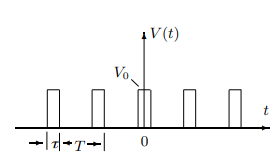
\includegraphics[width=0.7\linewidth]{3.6.1-1}}
		\caption{Прямоугольные импульсы}
		\end{minipage}
		\begin{minipage}[h]{0.5\linewidth}
		\center{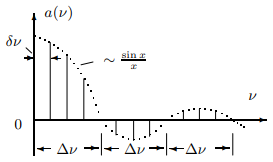
\includegraphics[width=0.7\linewidth]{3.6.1-2}}
		\caption{Спектр последовательности прямоугольных импульсов}
		\end{minipage}
	\end{figure}
		
	
	Назовем \textit{шириной спектра} $\Delta \omega$ расстояние от главного максимума ($\omega =0$) до первого нуля огибающей, возникающего при $n=\dfrac{2\pi}{\tau \Omega_{1}}$. При этом 

\begin{equation}\label{neopr}
	\Delta \omega \tau \backsimeq 2 \pi \;\;\;\;\; \text{или} \;\;\;\;\;
	\Delta \nu \Delta t \backsimeq 1
\end{equation}
		
	Полученное соотношение взаимной связи интервалов $\Delta \nu$ и $\Delta t$ является
	частным случаем соотношения неопределенности в квантовой механике.
	
	\item \textbf{Периодическая последовательность цугов} гармонического колебания $V_{0}\cos(\omega_{0}t)$ с длительностью цуга $\tau$ и периодом повторения $T$ (рис. 3).
	
	Функция $f(t)$ снова является четной относительно $t=0$. Коэффициент при $n$-й гармонике равен
	
	$$a_{n}=\dfrac{2}{T}\int\limits_{-\frac{\tau}{2}}^{\frac{\tau}{2}}V_{0}\cos(\omega_{0}t)\cos(n \Omega_{1} t)dt=V_{0}\dfrac{\tau}{T} \bigg(\dfrac{\sin[(\omega_{0}-n\Omega_{1})\frac{\tau}{2}]}{(\omega_{0}-n\Omega_{1})\frac{\tau}{2}}+\dfrac{\sin[(\omega_{0}+n\Omega_{1})\frac{\tau}{2}]}{(\omega_{0}+n\Omega_{1})\frac{\tau}{2}} \bigg)$$ 
	
	Зависимость для случая, когда $\frac{T}{\tau}$ равно целому числу, представлена на рис. 4. Сравнивая спектр последовательности прямоугольных импульсов и цугов мы видим, что они аналогичны, но их максимумы сдвинуты по частоте на величину $\omega_{0}$.
	
	\begin{figure}[h]
		\vspace{-5ex}
		\begin{minipage}[h]{0.5\linewidth}
		\center{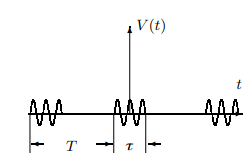
\includegraphics[width=0.7\linewidth]{3.6.1-3}}
		\caption{Последовательность цугов}
		\end{minipage}
		\begin{minipage}[h]{0.5\linewidth}
		\center{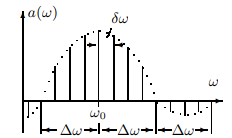
\includegraphics[width=0.7\linewidth]{3.6.1-4}}
		\caption{Спектр последовательности цугов}
		\end{minipage}
	\end{figure}	
	
	\item \textbf{Амплитудно-модулированные колебания.} Рассмотрим гармонические колебания высокой частоты $\omega_{0}$ , амплитуда которых медленно меняется по гармоническому закону с частотой $\Omega$ ($\Omega \ll \omega_{0})$) (рис. 5):
	
	$$f(t)=A_{0}[1+m\cos\Omega t]\cos \omega_{0}t.$$
	
	Коэффициент $m$ называют \textbf{глубиной модуляции}. При $m<1$ амплитуда колебаний меняется от минимальной $A_{min}=A_{0}(1-m)$ до максимальной $A_{max}=A_{0}(1+m).$ Глубина модуляции может быть представлена в виде
	
\begin{equation}\label{m}
	 m=\dfrac{A_{max}-A_{min}}{A_{max}+A_{min}}
\end{equation}
	
	Простым тригонометрическим преобразованием можно найти спектр амплитудно - модулированных колебаний:
	\\
\begin{equation}\label{a}
	f(t)=A_{0}\cos(\omega_{0} t)+\dfrac{A_{0}m}{2}\cos(\omega_{0}+\Omega)t+\dfrac{A_{0}m}{2}\cos(\omega_{0}-\Omega)t.
\end{equation}
	
	\begin{figure}[h]
		\vspace{-1ex}
		\begin{minipage}[h]{0.5\linewidth}
		\center{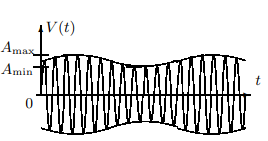
\includegraphics[width=0.7\linewidth]{3.6.1-5}}
		\caption{Модулированные гармонические колебания}
		\end{minipage}
		\begin{minipage}[h]{0.5\linewidth}
		\center{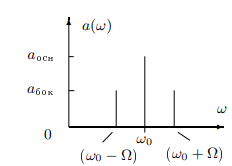
\includegraphics[width=0.7\linewidth]{3.6.1-6}}
		\caption{Спектр модулированных гармонических колебаний}
		\end{minipage}
	\end{figure}
		
		
		Спектр таких колебаний содержит три составляющих  основную
		компоненту и две боковых (рис. 6). Первое слагаемое в правой части представляет собой исходное немодулированное колебание
		с основной (несущей) частотой $\omega_{0}$ и амплитудой $a_{осн} = A_{0}$ . Второе и третье слагаемые соответствуют новым гармоническим колебаниям с частотами $\omega_{0} + \Omega$ и $\omega_{0} - \Omega$. Амплитуды этих двух колебаний одинаковы и составляют $\dfrac{m}{2}$ от амплитуды немодулированного колебания:
		$a_{бок} = \dfrac{A_{0}m}{2}$. Начальные фазы всех трех колебаний одинаковы.
	\end{enumerate}

	\subsection{Методика измерений}
	
	Для исследования спектров в работе используется гетеродинный анализатор спектра типа СК4-56. Упрощённая структурная схема, поясняющая последовательный супергетеродинный метод спектрального анализа внешнего сигнала, изображена на риc. 7.
	
\begin{figure}[H]
	\begin{center}
		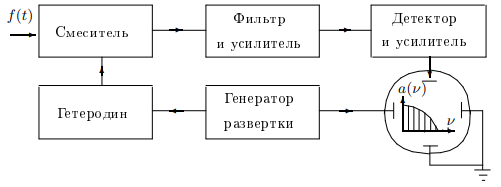
\includegraphics[width=15cm, height=4cm]{3.6.1-7}
		\caption{Структурная схема анализатора спектра}
	\end{center}
\end{figure}
	
	Восстановление спектрального состава заданным периодом f(t) происходит периодически с некоторым заданным периодом. Это время является периодом повторения пилообразного напряжения, которое вырабатывается генератором развёртки. Линейно нарастающее во времени напряжение с генератора развёртки подаётся на гетеродин, который генерирует переменное напряжение с частотой пропорциональной этому напряжению, но с постоянной амплитудой. При изменении пилообразного напряжения от нуля до некоторого максимального значения частота сигналов, вырабатываемых гетеродином, изменяется в пределах от 128 до 188 кГц. Исследуемый сигнал f(t) и переменное напряжение с гетеродина одновременно поступают на смеситель. При нелинейном сложении этих колебаний на выходе смесителя возникают сигналы суммарной и разностной частоты. Для анализа используется только разностный сигнал.
	
	Со смесителя сигнал поступает на фильтр, который настроен на частоту 128 кГц. Таким образом мы "извлекаем" из спектра входного сигнала f(t) переменное напряжение с частотой равной разности частот гетеродина и фильтра. За время, равное периоду повторения пилообразного напряжения, фильтр пропускает колебания с частотами от нуля до 60 кГц. Затем эти колебания детектируются, усиливаются и подаются на вертикальный вход электронно-лучевой трубки (ЭЛТ). Одновременно сигнал генератора развёртки поступает на горизонтальный вход ЭЛТ. На экране анализатора возникает, таким образом, график, изображающий зависимость амплитуды гармоник от частоты, т.е. фурье-спектр исследуемого сигнала. 

	\subsection{Экспериментальные установки}
	
	\begin{enumerate}
		
		\item \textbf{Экспериментальная установка А} для исследования спектра периодической последовательности прямоугольных импульсов представлена на рис. 8. Сигнал с выхода генератора прямоугольных импульсов Г5-54 подается на вход анализатора спектра и одновременно  на вход Y осциллографа. С генератора импульсов на осциллограф подается также сигнал синхронизации, запускающий ждущую развертку осциллографа. При этом на экране осциллографа можно наблюдать саму последовательность прямоугольных импульсов, а на экране ЭЛТ анализатора спектра  распределение амплитуд спектральных составляющих этой последовательности.
		
\begin{figure}[H]
	\begin{center}
		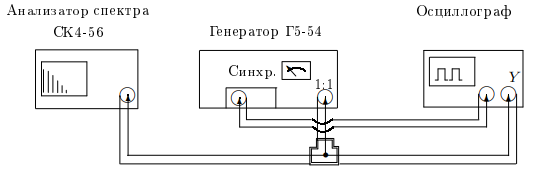
\includegraphics[width=15cm, height=4cm]{3.6.1-8}
		\caption{Схема для исследования спектра периодической последовательности прямоугольных импульсов}
	\end{center}
\end{figure}		
		
		\item \textbf{Экспериментальная установка Б} для исследования спектра периодической последовательности цугов гармонических колебаний (рис. 9) Генератор Г6-34 вырабатывает синусоидальные колебания высокой частоты. На вход АМ (амплитудная модуляция) генератора Г6-34 подаются прямоугольные импульсы с генератора Г5-54 и синусоида модулируется - "нарезается" на отдельные куски - цуги. Эти цуги с выхода генератора Г6-34 поступают на вход спектроанализатора и одновременно на вход Y осциллографа. Сигнал синхронизации подается на осциллограф с генератора импульсов.
		
\begin{figure}[H]
	\vspace{-5ex}
	\begin{center}
		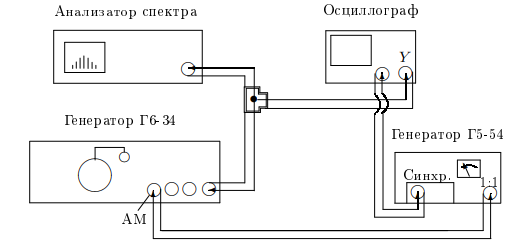
\includegraphics[width=15cm, height=6cm]{3.6.1-9}
		\caption{Схема для исследования спектра периодической последовательности цугов высокочастотных колебаний}
	\end{center}
\end{figure}
	
		\item \textbf{Экспериментальная установка В} для исследования амплитудно - модулированного сигнала (рис. 10). В генератор сигналов встроен модуляционный генератор, который расположен в левой части Г6-34. Синусоидальный сигнал с частотой модуляции $f_{мод}=1$ кГц подается с модуляционного генератора на вход АМ (амплитудная модуляция) генератора, вырабатывающего синусоидальный сигнал высокой частоты (частота несущей $\nu_{0}=25$ кГц). Амплитудно-модулированный сигнал с основного выхода генератора поступает на осциллограф и на анализатор спектра. 

\begin{figure}[H]
	\begin{center}
		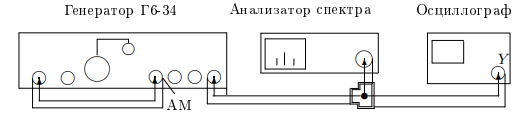
\includegraphics[width=15cm, height=4cm]{3.6.1-10}
		\caption{Схема для исследования спектра высокочастотного гармонического сигнала, промодулированного по амплитуде низкочастотным гармоническим сигналом}
	\end{center}
\end{figure}
		
	\end{enumerate}

  	\section{Ход работы}
  	
\end{document}